\chapter{Leveraging structured forest for segmentation}
\label{Chapter4}
\settocdepth{paragraph}
Given an edge detection result, various methods could be employed to obtain image segmentation.  One approach is to try and identify all possible boundaries of segmentation regions, based on the probability of boundary score produced by the edge detector. Those boundaries %, called \textit{watershed pixels}, 
finely partition the image pixel graph (see \sref{sec:ch3-watershed} for a description of the \textit{watershed transform} which we will use). The regions closed by them constitute an oversegmentation of the image. Different tasks require segmentation at different level of detail. It is useful, therefore, to be able to obtain coarser segmentations as well. 
By reasoning about the salience of region boundaries, one could construct a \textit{hierarchy of segmentations} (see \sref{sec:ch3-UCM} for details on the UCM). Going up the hierarchy corresponds to coarsening the segmentation by merging neighbouring regions which are separated by a weak boundary. To establish the order in which to merge the regions, we must be able to tell weak from strong boundaries. We want to associate a \textit{score} with every possible region boundary, which score should reflect the strength of that intervening boundary.

\textbf{Structured voting:} To score the region boundaries we take a patch comparison approach. The edge detector which we employ, Structured edge (SE) by Doll\'ar~\etal~\cite{DollarICCV13edges}, associates a segmentation to every patch centred around a pixel location in the image - its most likely segmentation. The possible region boundaries locations are obtained by a watershed transformation on the output of this detector. For the same location we attain a patch from the watershed locations image. We then explore strategies to compare those two patches and score the similarity between them, a higher score meaning higher local evidence for boundary. We call those \textbf{watershed weighting strategies}. The choice of such an approach defines how we conduct our \textbf{Structured voting (SV)}.

\textbf{How to vote? Two essentials:} We identify two important points in order to be able to score the two patches just described. 
Firstly, one being a local segmentation, and the other - a local oversegmentation, they are quite dissimilar. Therefore, one patch needs to be sensibly \textbf{transformed}, so that the two patches are comparable. 
Secondly, given that the two patches are comparable, what \textbf{scoring function} should be employed? We cast the problem of comparing two segmentation patches as a segmentation benchmark problem. Various boundary- and region-based metrics have been proposed for the task of evaluating image segmentation. We analyse the theoretical properties of some, and use a suitable %reasonable 
subset of them in our practical experiments. 
So a watershed weighting strategy has two aspects - making the patches sufficiently similar to compare, and choosing a scoring function to compare them.

\textbf{Pipeline:} In the terms of the framework of Arbel\'aez~\etal~\cite{Arbelaez11} - gPb-OWT-UCM, we propose to use SE instead of gPb as an edge detector. Further, we replace the Oriented watershed transform (OWT) by SV to obtain scored region boundary locations. Our image segmentation pipeline could then be titled \textbf{SE-SV-UCM}, see \fref{fig:SE-SV-UCM-pipeline}.

\begin{figure}[ht!]
\centering
 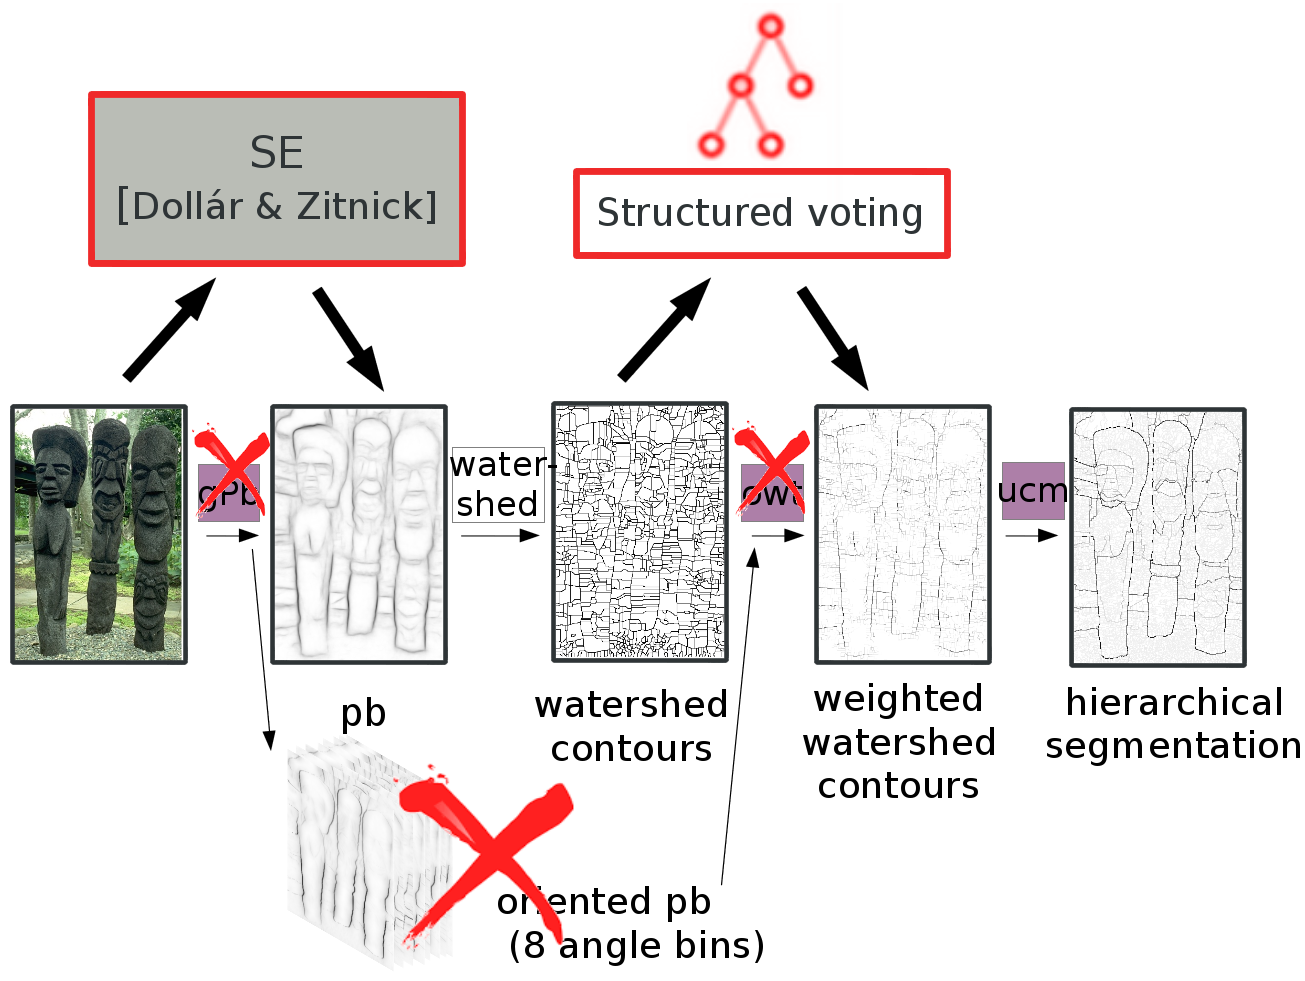
\includegraphics[width=1\textwidth]{images/SE-SV-UCM/SE-SV-UCM_pipeline.png}
\caption{Our SE-SV-UCM algorithm in the context of gPb-OWT-UCM pipeline, see \fref{fig:gPb-OWT-UCM-pipeline}.}
\label{fig:SE-SV-UCM-pipeline}
\end{figure}

In the rest of the chapter we describe our algorithm's pipeline. We finish with a discussion on practical issues concerning edge detection and image segmentation output format.

\section[First stage of the pipeline - Structured edge]{First stage of the pipeline - edge detection - Structured edge}
We employ the edge detector SE of~\cite{DollarICCV13edges,Dollar2015PAMI}.

\subsection{gPb vs. SE}
The gPb algorithm uses a combination of carefully designed features - the gradients, each at 3 scales of: 1) texture, 2) brightness, and 3) colour (a total of 9 channels). As Doll\'ar reports in~\cite{DollarICCV13edges}, despite a high score on the BSDS500 dataset, gPb performs poorly when tested on other datasets. This is potentially a symptom of over-tuning of the algorithm to the dataset.

Beside being heavily-engineered, in terms of detection speed it does not come close to the real-time performance of SE.

The chief reason for using SE for us, however, is that this edge detector can provide as a by-product the intermediate most likely-segmentations that it has predicted per location in the image. This is important information about the local edge structure that we will build on when developing our Structured voting (SV).

\section{Second stage of the pipeline - Structured voting}
\label{sec:ch4-SE-SV-UCM_SV_details}
The goal of SV is to propose a suitable way of associating a score with each of the {\it watershed pixels} (the computed possible locations of boundary). Inspired by the ``local patch as a means of capturing context'' philosophy of previous works~\cite{Dollar2006supervised,LimZD13,DollarICCV13edges}, we take a patch comparison approach.

\subsection{Weighting the watershed contours} %locations}
The SE provides us ``for free'' with the best segmentation patches - local decisions that the trees of the decision forest have made {\bf on all locations} of the image. The size of those medoid tree leaf patches (as well as of all structured forest segmentation patches) is $16\times 16$ pixels.

\settocdepth{subsection}
\subsubsection{Casting a single vote}
\settocdepth{paragraph}
We only cast votes on the {\bf watershed contour pixels}. To this end, we crop from the watershed superpixels image a patch (the same size as the tree leaves patches), such that its centre is a potential boundary pixel. We want to quantify the strength of this boundary. 
% We crop, centred around the same location, a patch of the same size.

That we do by comparing the two - the watershed pixels patch and a tree leaf patch centred around the same location. This comparison gives us a score, which we associate with the chosen location on the watershed contours.

\settocdepth{subsection}
\subsubsection{Votes averaging}
\settocdepth{paragraph}
A total number of $T=4$ votes are cast per watershed pixel, and we take the mean of those. To further denoise the voting and give our votes a larger platform, % stage, dais, rostrum, podium
we average all votes per \textit{watershed arc}. The watershed arcs, as discussed in \sref{sec:ch3-OWT}, are edges of the watershed contours, which are fairly consistent in their orientation. They are obtained by recursively subdividing the region boundaries of the watershed until the approximation given by the straight line through the end of the watershed arc is a sufficiently good one. % TODO artefact from the OWT

\subsection{Comparing a structured forest patch to a watershed patch}
\begin{figure}[ht!]
\centering
 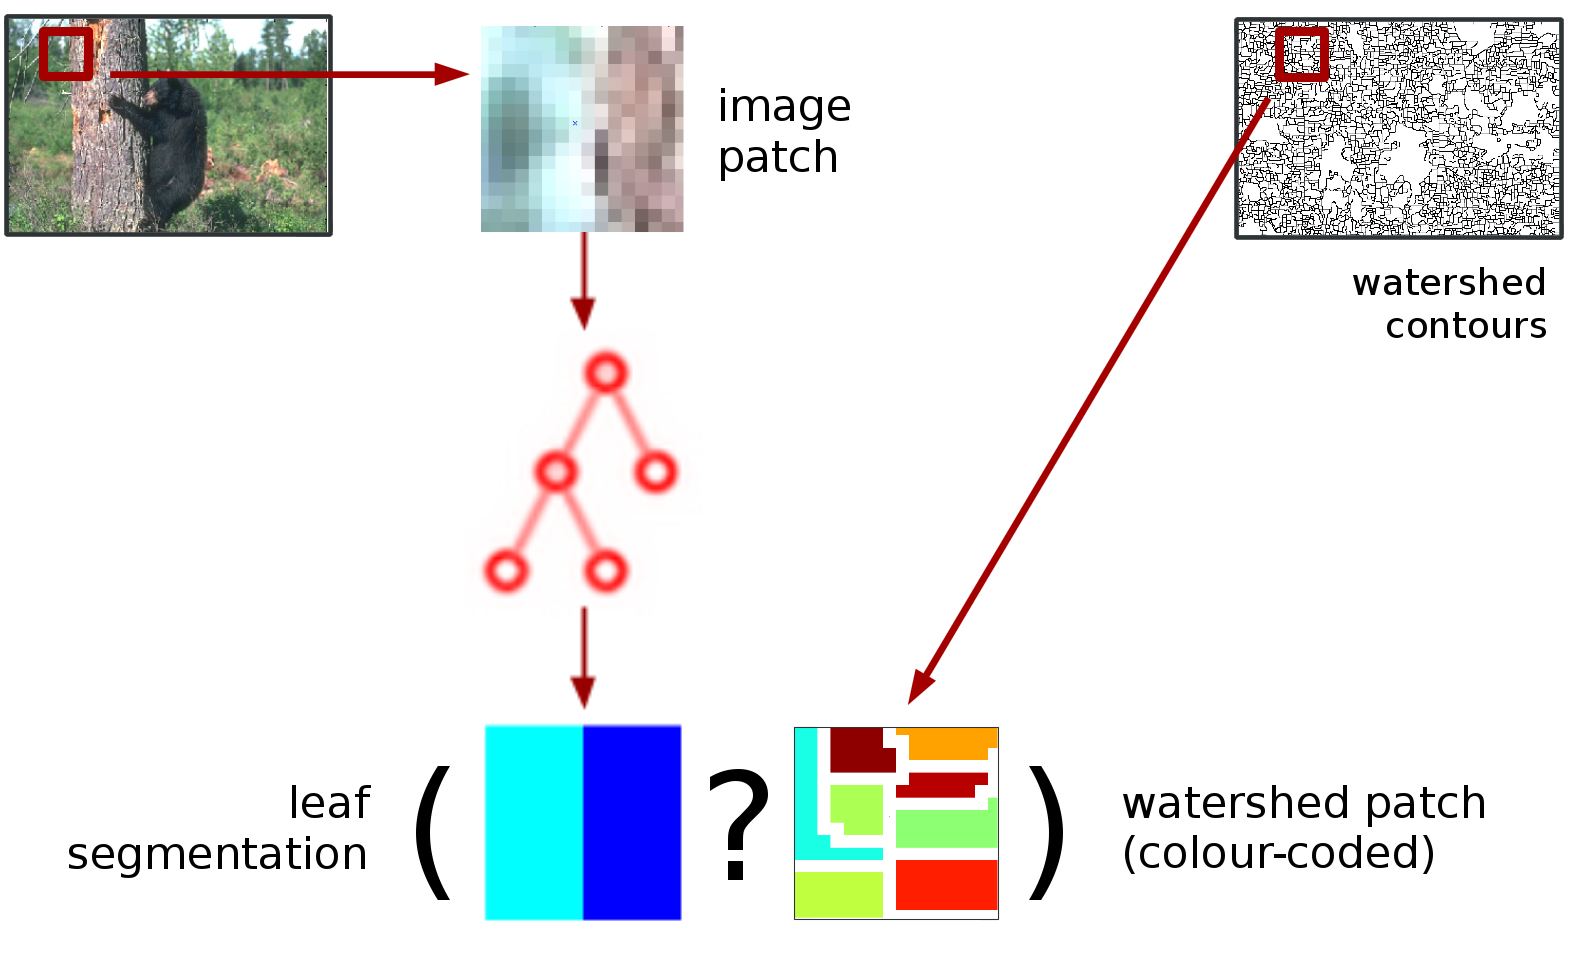
\includegraphics[width=1\textwidth]{images/SE-SV-UCM/weighting-the-watershed-contours-two-patches.png}
\caption[Structured voting essence: a comparison of two patches]{We have the task of comparing and scoring the similarity of two patches - a \textbf{decision tree leaf segmentation} and a \textbf{watershed oversegmentation}.}
\label{fig:weighting-the-watershed-contours}
\end{figure}

For a specific location one tree of the structured forest predicts a segmentation. From the watershed we have a corresponding patch, see \fref{fig:weighting-the-watershed-contours}. As mentioned already, there are two aspects to scoring their similarity: 1) making them suitable (\ie sufficiently similar) for comparison, and 2) choosing a function that can assess the agreement between the two patches as to the presence or absence of an edge.

\subsubsection{Patch transformations}
\label{sec:ch4-patch-transformations}
To appreciate the necessity of making the two types of segmentation patches comparable, look at \fref{fig:watershed-and-leaf-patches} which features a selection of watershed and tree leaf patches.

\textbf{Watershed patch:} The watershed patch is an oversegmentation with an \textbf{explicit boundary of size 1 pixel} between the segments.

\textbf{Tree leaf patch:} The segmentation patches from the Structured forest are the learnt best segmentation for the given location in the image (based on the features computed from a cropped image patch). They are patches ``seen'' by the forest during the training phase. Since the SE algorithm uses \textbf{supervised learning}, the patches are cropped from the ground truth annotated segmentations. 
For the BSDS500 dataset, which we use, the segmentation labels  are assigned by humans, and they are never oversegmentations. In \textsection~\ref{sec:ch5-BSDS500-dataset} we give details about this dataset, and \fref{fig:BSDS-annotations} has an example image and its annotations.

For a $16\times 16$ pixels local segmentation patch there rarely are more than \textbf{2 or 3 segments}. 
A ground truth segmentation in this dataset constitutes a labelling of the pixels, so that homogeneous regions - superpixels, are formed. The labels are unique and the \textbf{boundary between segments is implicit}.

\textbf{Tree leaf background patches:} Note that in~\ref{fig:watershed-and-leaf-patches} we only show examples of \textbf{non-background} patches. Background patches would contain a single region - the whole patch. Clearly, %Evidently, 
they present local evidence of lack of boundary.

\begin{figure}[ht!]
\begin{center}
  \begin{tabular}{ c c c c c c }
  
\includegraphics[width=0.13\textwidth,frame]{images/SE-SV-UCM/watershed-patches/watershed-patch1.png} &  
\includegraphics[width=0.13\textwidth,frame]{images/SE-SV-UCM/watershed-patches/watershed-patch2.png} &
  
\includegraphics[width=0.13\textwidth,frame]{images/SE-SV-UCM/watershed-patches/watershed-patch3.png} &
  
\includegraphics[width=0.13\textwidth,frame]{images/SE-SV-UCM/leaf-patches/leaf-patch2.png} & % 
\includegraphics[width=0.13\textwidth,frame]{images/SE-SV-UCM/leaf-patches/leaf-patch1.png} & % too similar to leaf-patch4.png
  
\includegraphics[width=0.13\textwidth,frame]{images/SE-SV-UCM/leaf-patches/leaf-patch13.png} &
  
\includegraphics[width=0.13\textwidth,frame]{images/SE-SV-UCM/leaf-patches/leaf-patch4.png} \\

  
\includegraphics[width=0.13\textwidth,frame]{images/SE-SV-UCM/watershed-patches/watershed-patch4.png} &
  
\includegraphics[width=0.13\textwidth,frame]{images/SE-SV-UCM/watershed-patches/watershed-patch5.png} &
  
\includegraphics[width=0.13\textwidth,frame]{images/SE-SV-UCM/watershed-patches/watershed-patch6.png} &
  
\includegraphics[width=0.13\textwidth,frame]{images/SE-SV-UCM/leaf-patches/leaf-patch3.png} &
  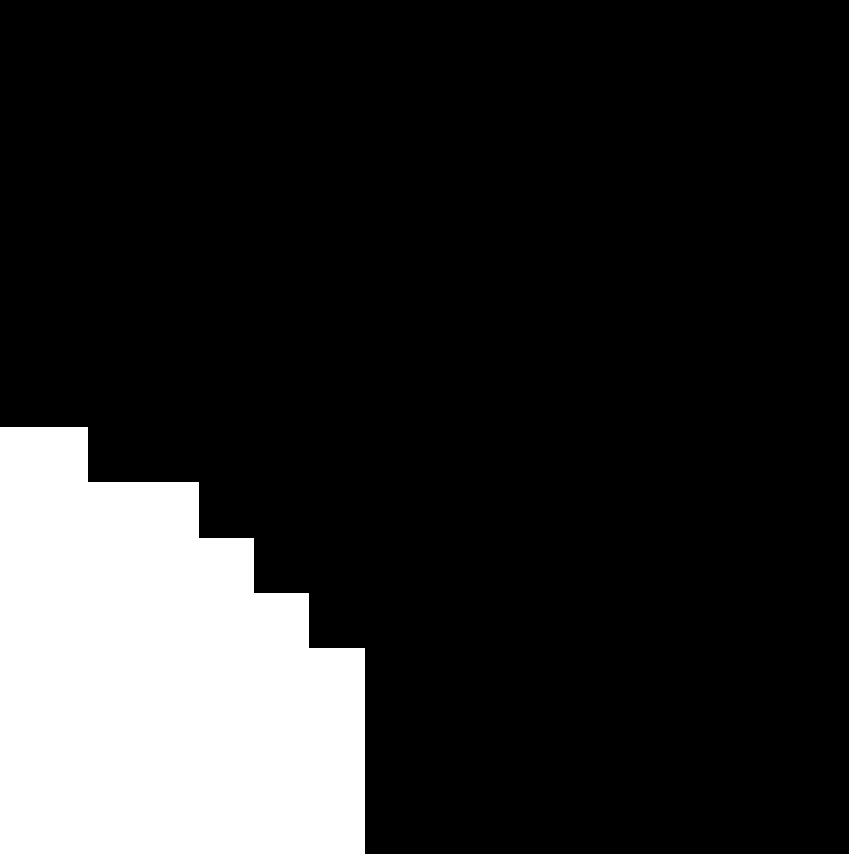
\includegraphics[width=0.13\textwidth,frame]{images/SE-SV-UCM/leaf-patches/leaf-patch5.png} &
  
\includegraphics[width=0.13\textwidth,frame]{images/SE-SV-UCM/leaf-patches/leaf-patch6.png} \\

  
\includegraphics[width=0.13\textwidth,frame]{images/SE-SV-UCM/watershed-patches/watershed-patch9.png} &
  
\includegraphics[width=0.13\textwidth,frame]{images/SE-SV-UCM/watershed-patches/watershed-patch7.png} &
  
\includegraphics[width=0.13\textwidth,frame]{images/SE-SV-UCM/watershed-patches/watershed-patch8.png} &
  
\includegraphics[width=0.13\textwidth,frame]{images/SE-SV-UCM/leaf-patches/leaf-patch7.png} &
  
\includegraphics[width=0.13\textwidth,frame]{images/SE-SV-UCM/leaf-patches/leaf-patch8.png} & % 
\includegraphics[width=0.13\textwidth,frame]{images/SE-SV-UCM/leaf-patches/leaf-patch9.png} \\ % too similar to leaf-patch8.png
  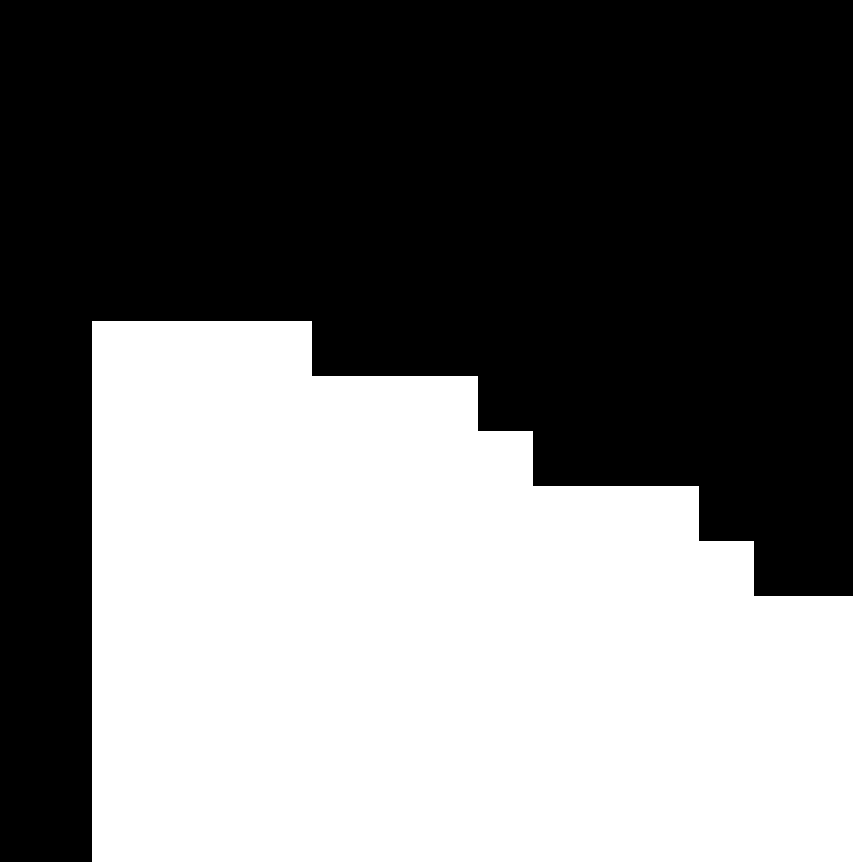
\includegraphics[width=0.13\textwidth,frame]{images/SE-SV-UCM/leaf-patches/leaf-patch18.png} \\

  
\includegraphics[width=0.13\textwidth,frame]{images/SE-SV-UCM/watershed-patches/watershed-patch10.png} &
  
\includegraphics[width=0.13\textwidth,frame]{images/SE-SV-UCM/watershed-patches/watershed-patch11.png} &
  
\includegraphics[width=0.13\textwidth,frame]{images/SE-SV-UCM/watershed-patches/watershed-patch12.png} &
  
\includegraphics[width=0.13\textwidth,frame]{images/SE-SV-UCM/leaf-patches/leaf-patch10.png} &
  
\includegraphics[width=0.13\textwidth,frame]{images/SE-SV-UCM/leaf-patches/leaf-patch11.png} &
  
\includegraphics[width=0.13\textwidth,frame]{images/SE-SV-UCM/leaf-patches/leaf-patch12.png} \\

  
\includegraphics[width=0.13\textwidth,frame]{images/SE-SV-UCM/watershed-patches/watershed-patch13.png} &
  
\includegraphics[width=0.13\textwidth,frame]{images/SE-SV-UCM/watershed-patches/watershed-patch14.png} &
  
\includegraphics[width=0.13\textwidth,frame]{images/SE-SV-UCM/watershed-patches/watershed-patch15.png} &
  
\includegraphics[width=0.13\textwidth,frame]{images/SE-SV-UCM/leaf-patches/leaf-patch-3-segms1.png} &
  
\includegraphics[width=0.13\textwidth,frame]{images/SE-SV-UCM/leaf-patches/leaf-patch-3-segms2.png} &
  
\includegraphics[width=0.13\textwidth,frame]{images/SE-SV-UCM/leaf-patches/leaf-patch-3-segms3.png} \\
  \end{tabular}
  % unused watershed patches: watershed-patch 16 17
  %
  % unused leaf patches: leaf-patch 1 9 14 15 16 17
  %                      leaf-patch-3-segms 4 5 6 7 
  % leaf-patch-_maybe_problematic - two separate segments with the same label % do we handle that? hmmm....
\end{center}
\caption{Examples of {\bf watershed} patch segmentations (colour-coded on the {\bf left}; white pixels mark the explicit boundary) and structured decision {\bf tree leaf} patch segmentations (greyscale on the {\bf right}).}
\label{fig:watershed-and-leaf-patches}
\end{figure}

\paragraph{Greedy merge}\mbox{}\\\mbox{}\\ % force some space after the paragraph name
For this paragraph, please first have a look at \fref{fig:ws-greedy-merge}. Evidently merely converting the watershed oversegmentation to have implicit boundaries (from the original watershed patch segmentation - \fref{fig:sub:ws-greedy-merge-ws-colour-coded} to the segmentation labelling - \fref{fig:sub:ws-greedy-merge-ws-segments}) is not sufficient. The watershed is still very different from the target - the decision tree leaf patch (\fref{fig:sub:ws-greedy-merge-tree-leaf}), in the sense that it contains many more segments.

\subparagraph{Na\"{\i}ve greedy merge:} Our first attempt, which we call na\"{\i}ve greedy merge, suffered from the limitation of being overly 
greedy. The transformed watershed patch (see \fref{fig:sub:ws-greedy-merge-ws-naive-greedy-merge}) adapts itself excessively to the tree leaf segmentation which we use to guide the merging. As a consequence, it does not respect the fact that the watershed patch has a \textbf{boundary pixel in the middle}, hence, there must have been no less than two segments abutting its centre pixel.

\subparagraph{Fair greedy merge:} As a remedy, we propose a ``fairer'' greedy merge. It %uses heuristic to
aims for an optimal superpixels merge into segments, according to the structured tree patch (\fref{fig:sub:ws-greedy-merge-tree-leaf}). At the same time it still respects the condition that the central watershed pixel lies on a boundary between two regions. \fref{fig:sub:ws-greedy-merge-ws-fairer-greedy-merge} shows an example.

\begin{figure}[ht!]
\centering
 \subfigure[Input image]{%
  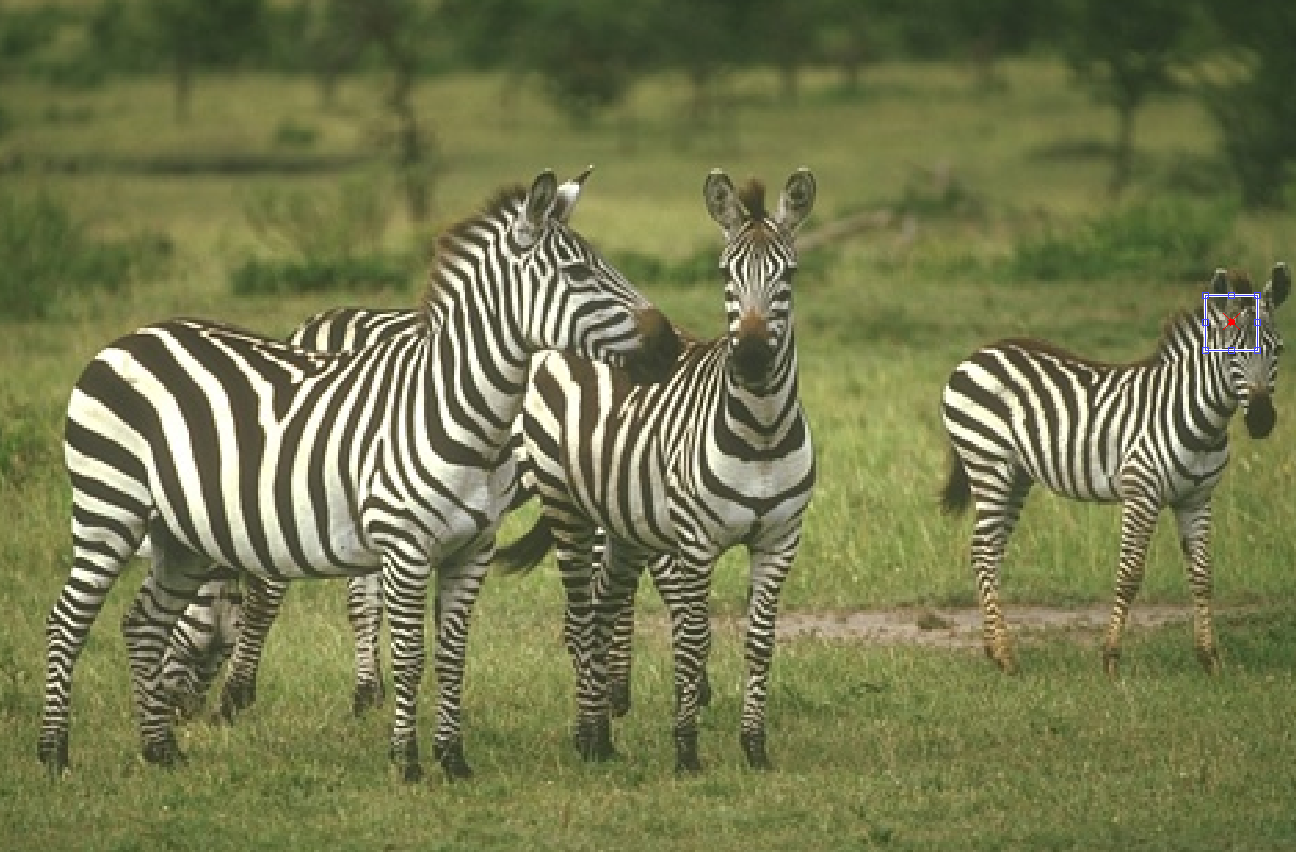
\includegraphics[width=0.5\textwidth]{images/SE-SV-UCM/ws-greedy-merge/zebras2.png}
 }
 \subfigure[Cropped image patch]{%
  
\includegraphics[width=0.2\textwidth]{images/SE-SV-UCM/ws-greedy-merge/selected-image-patch.png}
 }

 \subfigure[Cropped watershed patch]{%
  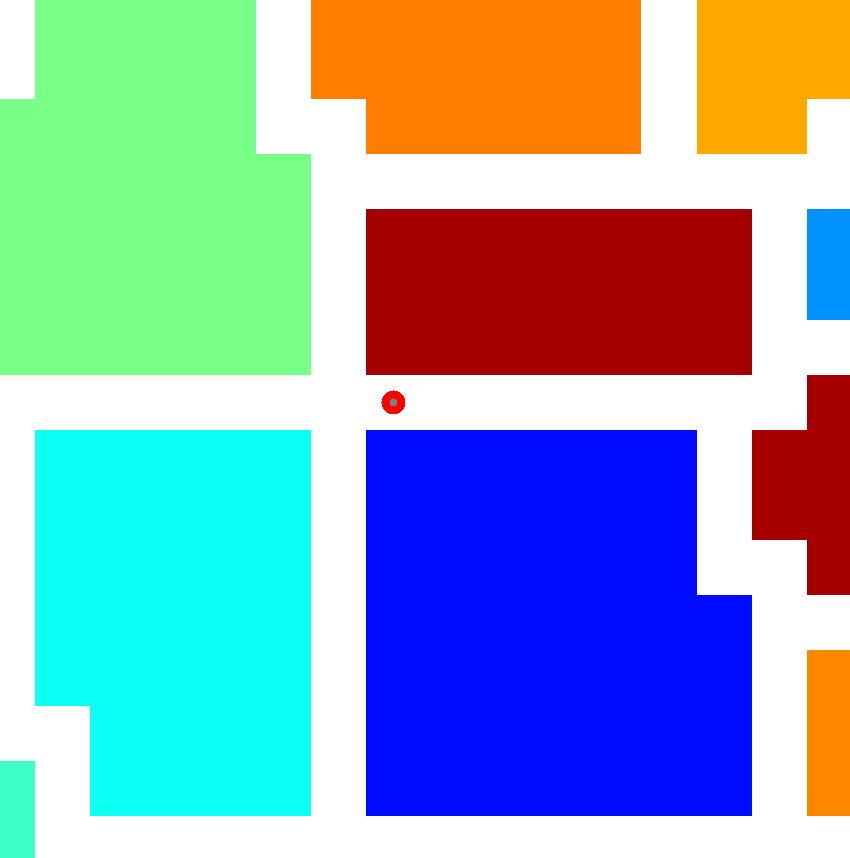
\includegraphics[width=0.2\textwidth,frame]{images/SE-SV-UCM/ws-greedy-merge/watershed-colour-coded.png}
  \label{fig:sub:ws-greedy-merge-ws-colour-coded}
 }
 \subfigure[Watershed patch with implicit region boundaries]{%
  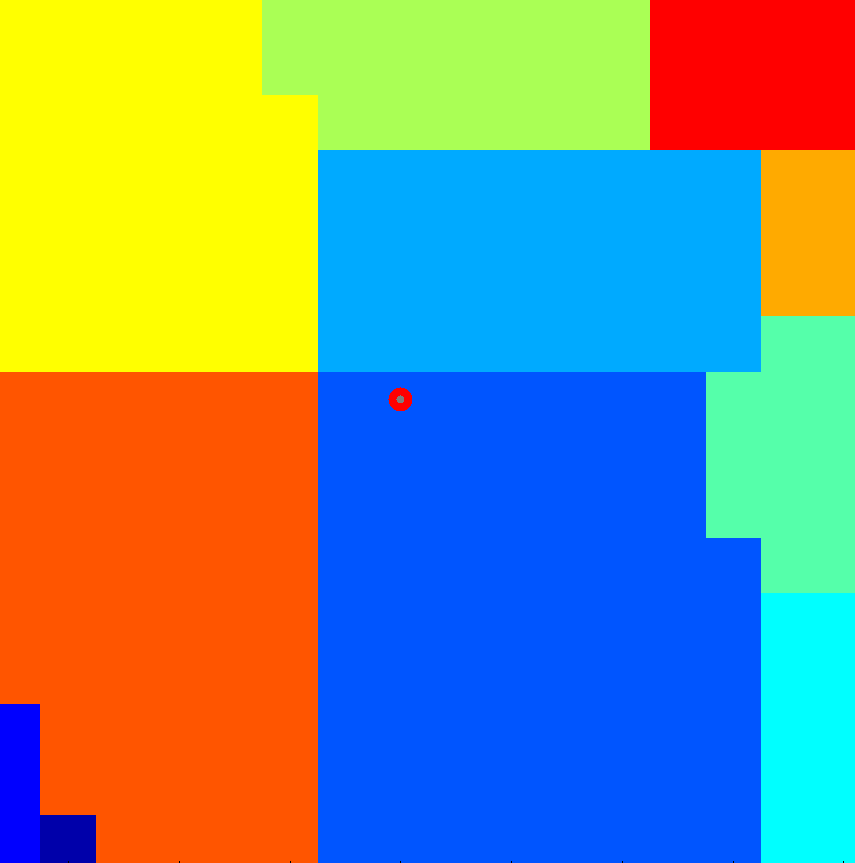
\includegraphics[width=0.2\textwidth,frame]{images/SE-SV-UCM/ws-greedy-merge/watershed-segments.png}
  \label{fig:sub:ws-greedy-merge-ws-segments}
 } \qquad\qquad\qquad\qquad\qquad

 \subfigure[Tree leaf segmentation patch that guides the merging]{%
  \fboxrule=2pt %border thickness
  \fcolorbox{red}{white}{\fboxrule=0.5pt 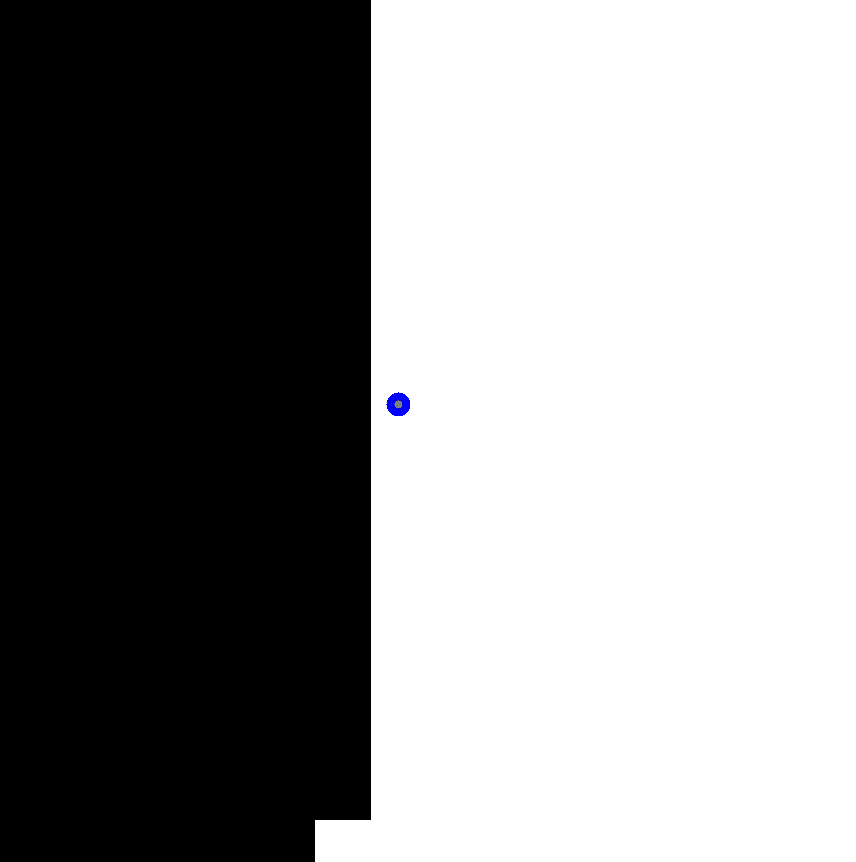
\includegraphics[width=0.2\textwidth,frame]{images/SE-SV-UCM/ws-greedy-merge/tree-leaf.png}}
  \label{fig:sub:ws-greedy-merge-tree-leaf}
 }
 \subfigure[Watershed patch {\bf na\"{\i}ve} greedy merge]{%
  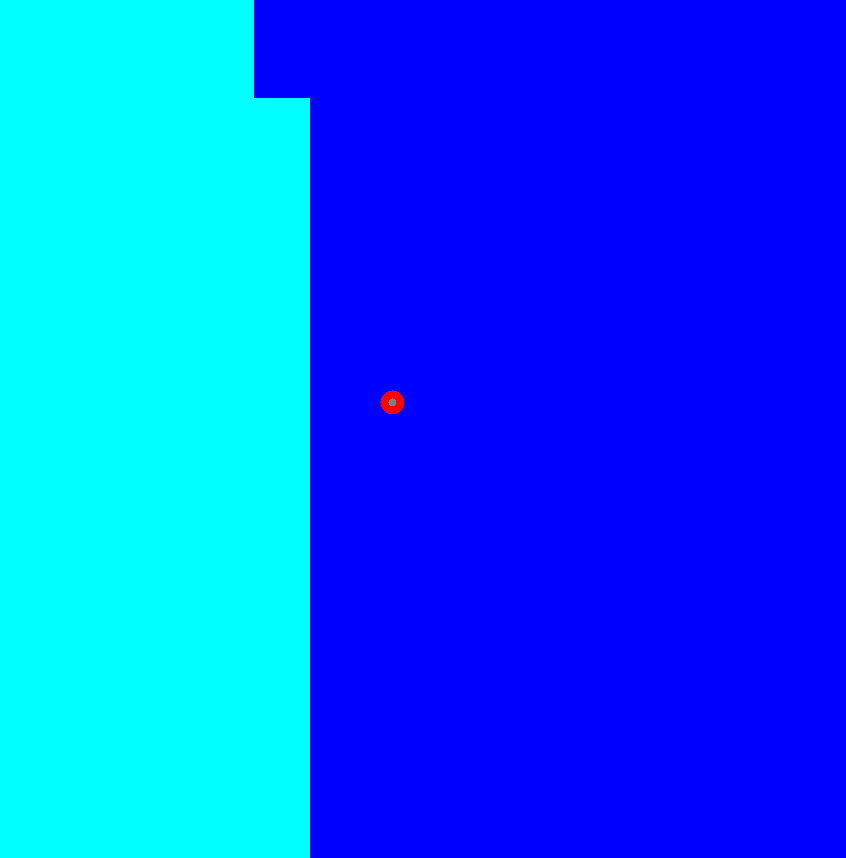
\includegraphics[width=0.2\textwidth,frame]{images/SE-SV-UCM/ws-greedy-merge/watershed-naive-greedy-merge.png}
  \label{fig:sub:ws-greedy-merge-ws-naive-greedy-merge}
 }
 \subfigure[Watershed patch {\bf fair} greedy merge]{%
  \fboxrule=2pt %border thickness
  \fcolorbox{green}{white}{\fboxrule=0.5pt 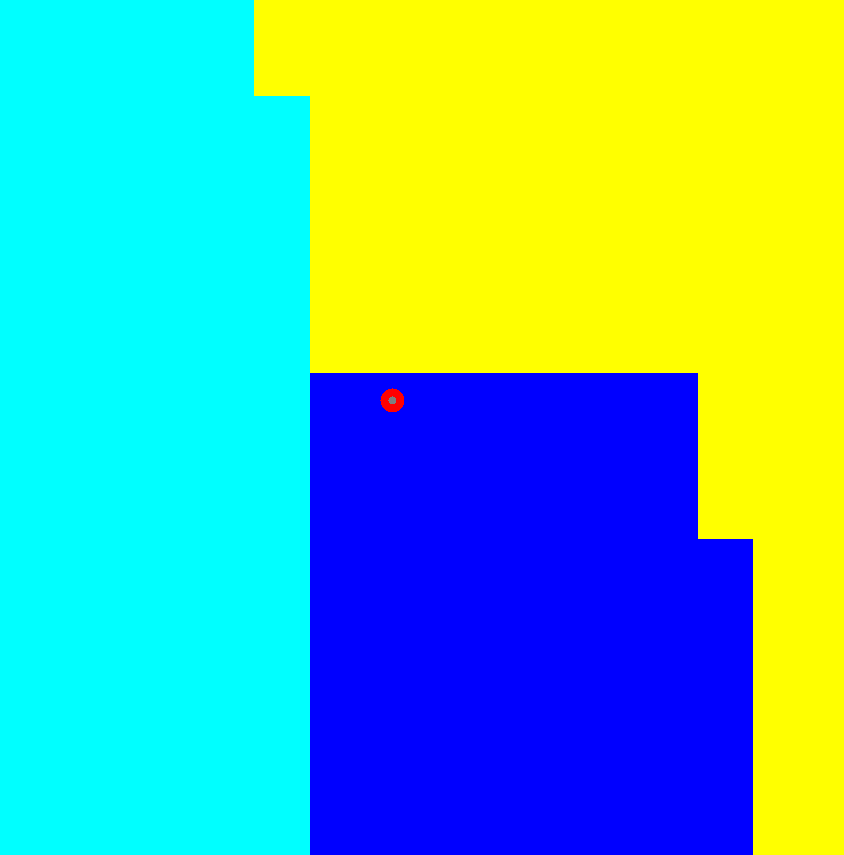
\includegraphics[width=0.2\textwidth,frame]{images/SE-SV-UCM/ws-greedy-merge/watershed-fairer-greedy-merge.png}}
  \label{fig:sub:ws-greedy-merge-ws-fairer-greedy-merge}
 }
\caption[{\bf Greedy merge} of watershed patch.]{{\bf Greedy merge} of watershed patch. The central pixel of the patches is marked, as it is important, see the text for details. The comparison is between a tree leaf patch (in red \protect\subref{fig:sub:ws-greedy-merge-tree-leaf}) and a watershed patch (in green \protect\subref{fig:sub:ws-greedy-merge-ws-fairer-greedy-merge}).}
\label{fig:ws-greedy-merge}
\end{figure}

\paragraph{Watershed arc}\mbox{}\\\mbox{}\\ % previously called ``just contour'' % region boundary
\label{par:ch4-watershed-arc}
See \fref{fig:ws-just-contour} for an example. Here we take into account only the underlying region boundary, on which the central pixel of the watershed patch is.

\textbf{Watershed arc:} We recursively subdivide this boundary until a \textbf{watershed arc} is obtained, \fref{fig:sub:ws-just-contour-watershed-just-contour}, whose shape could be sufficiently accurately approximated by the straight line through the arc's end points. We described this subdivision in Section~\ref*{sec:ch3-OWT}~\ref{par:ch3-watershed-arc}. See also \fref{fig:Arbelaez09-watershed-arcs}.

\begin{figure}[ht!]
 \centering
 \subfigure[Input image]{%
  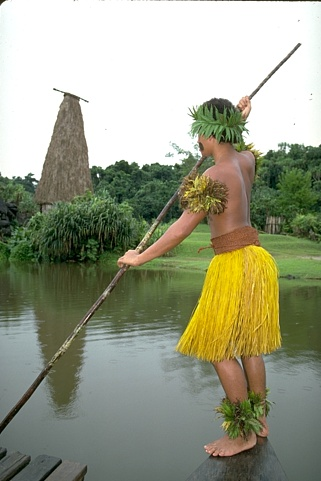
\includegraphics[width=0.25\textwidth]{images/examples/hawaii/hawaii.jpg}
 }
 \subfigure[Detail of the watershed image - region boundaries and their straight-line approximations]{%
  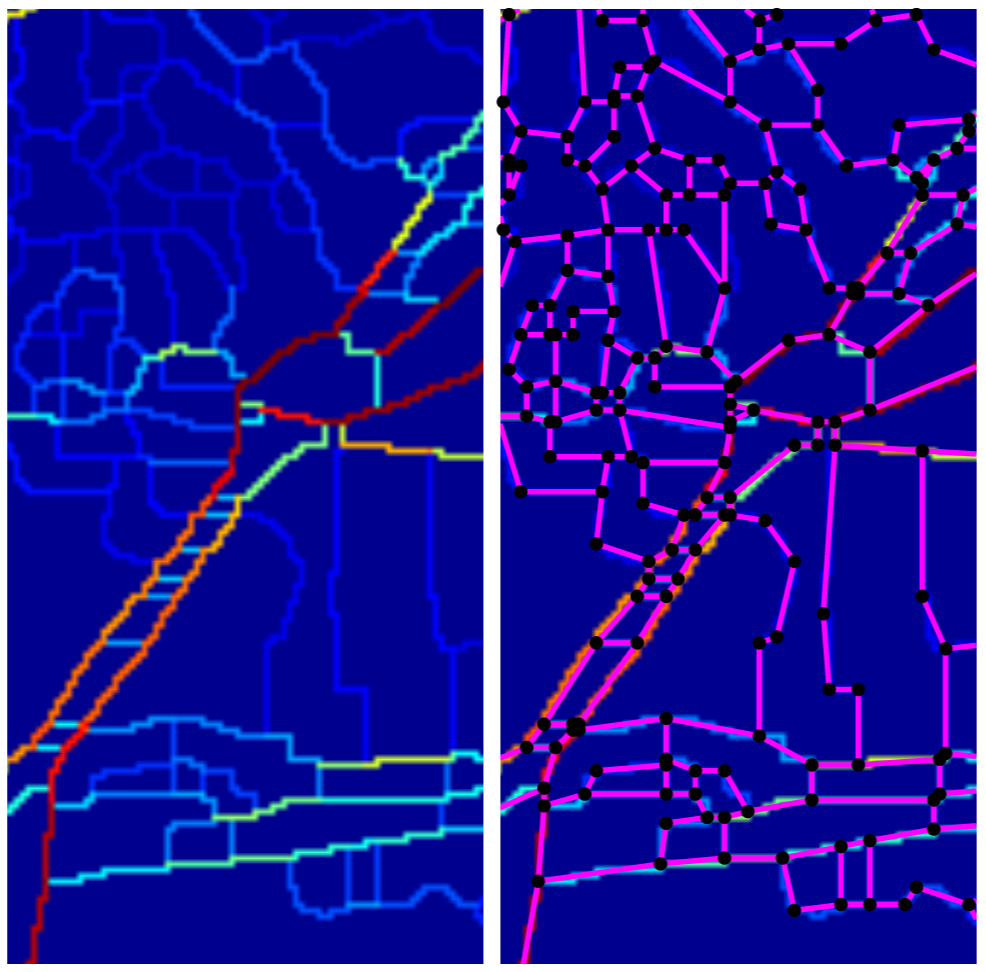
\includegraphics[width=0.71\textwidth]{images/SE-SV-UCM/Arbelaez09-hawaii-watershed-arcs.png}
 }
 \caption[Region boundary subdivision into watershed arcs]{{\bf Region boundary subdivision into {\bf watershed arcs}} (courtesy of \cite{Arbelaez09}). {\bf Middle:} Colour-coded are given the full region boundaries (these are the initial watershed arcs before subdivision is performed). {\bf Right:} The final set of watershed arcs is confined by % enclosed between 
 the end vertices of the approximating line fragments (shown in magenta).}
 \label{fig:Arbelaez09-watershed-arcs}
\end{figure}

\textbf{Tree leaf segmentation transformation:} As the resulting watershed patch is not a segmentation - often it would contain just an edge, and not a contour, we cannot keep the tree leaf as segmentation labelling (see \fref{fig:sub:tree-leaf-segments}. Instead we transform it, making the boundaries between the regions explicit, as in \fref{fig:sub:tree-leaf-boundaries}.

\textbf{Edge detection comparison:} Consequently, we would need a boundary evaluation metric to compare the two, as the watershed patch, when transformed, won't necessarily contain regions. Details on the metric that we will use are given in Section~\ref*{sec:ch4-boundary-and-region-metrics-maths}~\ref{par:ch4-BPR-maths}.

Note that, unlike with \textit{greedy merge}, none of the transformations given here depend on the other patch. The watershed arc is uniquely determined by the pixel around which the watershed patch is centred.

\begin{figure}[ht!]
\begin{center}
 \subfigure[Input image]{%
  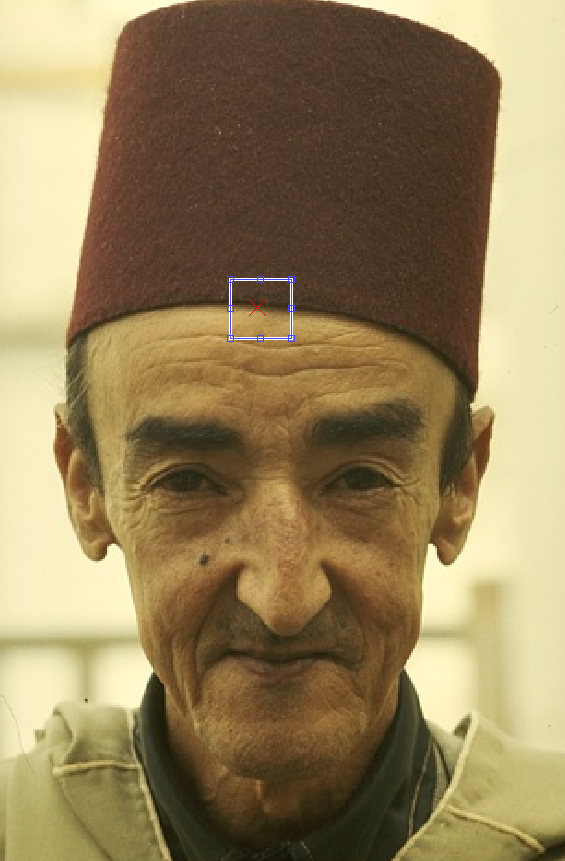
\includegraphics[width=0.14\textwidth]{images/SE-SV-UCM/ws-just-contour/old_man.png}
 }
 \subfigure[Cropped image patch]{%
  
\includegraphics[width=0.15\textwidth]{images/SE-SV-UCM/ws-just-contour/selected-image-patch.png}
 }
 \subfigure[Matching %Corresponding 
 watershed patch]{%
  
\includegraphics[width=0.15\textwidth,frame]{images/SE-SV-UCM/ws-just-contour/watershed-colour-coded.png}
  \label{fig:sub:ws-just-contour-watershed-colour-coded}
 }
 \subfigure[\protect\subref{fig:sub:ws-just-contour-watershed-colour-coded}~transformed - just an arc]{%
  \fboxrule=2pt %border thickness
  \fcolorbox{green}{white}{\fboxrule=0.5pt 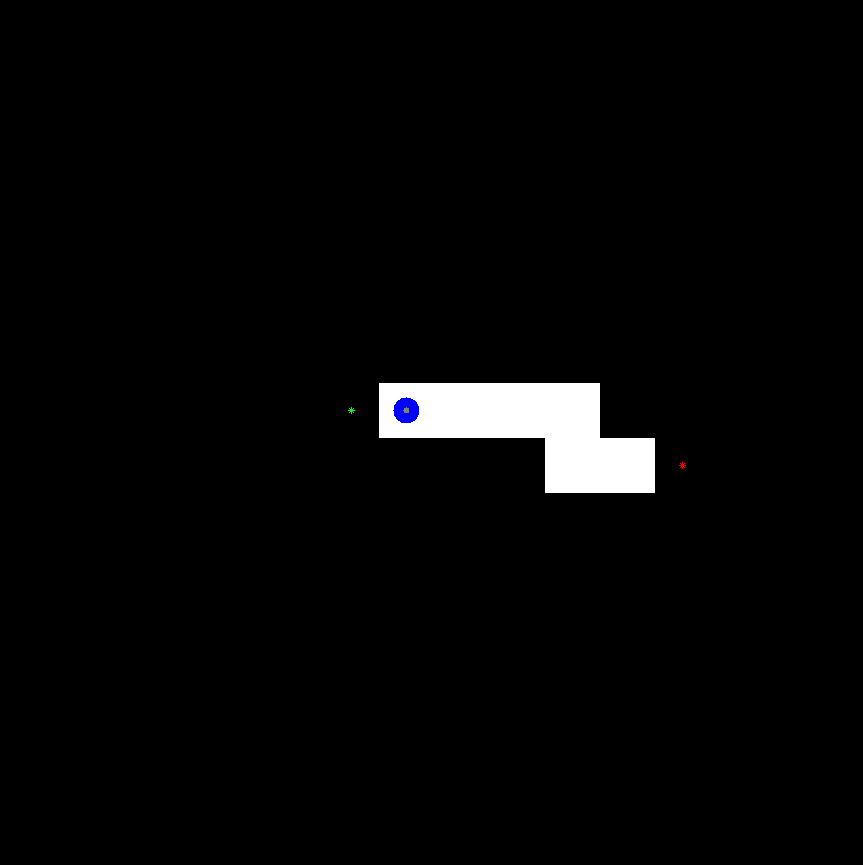
\includegraphics[width=0.15\textwidth,frame]{images/SE-SV-UCM/ws-just-contour/watershed-just-contour.png}}
  \label{fig:sub:ws-just-contour-watershed-just-contour}
 }

 % for the next 8 images, width=0.15 also works
 \subfigure[The 4 tree leaf segmentations]{%
  \begin{tabular}{ c c c c }
  Tree 1 & Tree 2 & Tree 3 & Tree 4 \\
  
\includegraphics[width=0.13\textwidth,frame]{images/SE-SV-UCM/ws-just-contour/tree1-seg.png} &
  
\includegraphics[width=0.13\textwidth,frame]{images/SE-SV-UCM/ws-just-contour/tree2-seg.png} &
  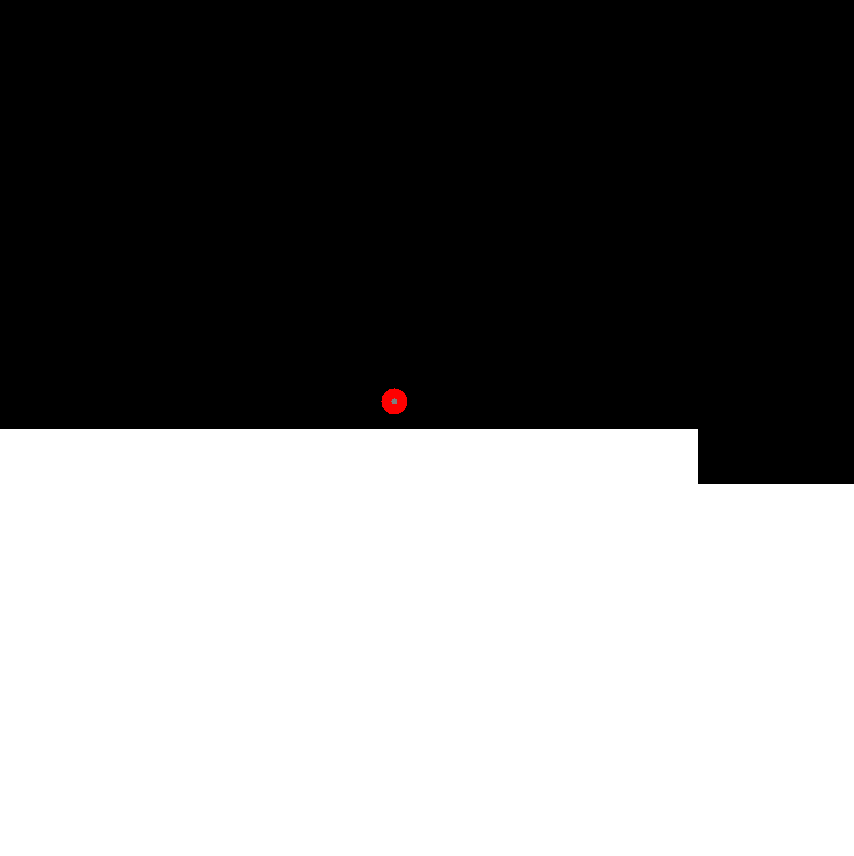
\includegraphics[width=0.13\textwidth,frame]{images/SE-SV-UCM/ws-just-contour/tree3-seg.png} &
  \includegraphics[width=0.13\textwidth,frame]{images/SE-SV-UCM/ws-just-contour/tree4-seg.png} \\
  \end{tabular}
  \label{fig:sub:tree-leaf-segments}
 }

 \subfigure[\protect\subref{fig:sub:tree-leaf-segments}~transformed to boundaries]{
  \begin{tabular}{ c c c c }
  {\fboxrule=2pt \fcolorbox{red}{white}{\fboxrule=0.5pt \includegraphics[width=0.13\textwidth,frame]{images/SE-SV-UCM/ws-just-contour/tree1-bdry.png}}} &
  {\fboxrule=2pt \fcolorbox{red}{white}{\fboxrule=0.5pt \includegraphics[width=0.13\textwidth,frame]{images/SE-SV-UCM/ws-just-contour/tree2-bdry.png}}} &
  {\fboxrule=2pt \fcolorbox{red}{white}{\fboxrule=0.5pt \includegraphics[width=0.13\textwidth,frame]{images/SE-SV-UCM/ws-just-contour/tree3-bdry.png}}} &
  {\fboxrule=2pt \fcolorbox{red}{white}{\fboxrule=0.5pt \includegraphics[width=0.13\textwidth,frame]{images/SE-SV-UCM/ws-just-contour/tree4-bdry.png}}} \\
  \end{tabular}
  \label{fig:sub:tree-leaf-boundaries}
  }
\end{center}
\caption[Watershed transformation to just {\bf region boundary}]{Watershed transformation to just {\bf region boundary}. The comparison is between the watershed patch (in green \protect\subref{fig:sub:ws-just-contour-watershed-just-contour}) and a tree leaf patch (in red \protect\subref{fig:sub:tree-leaf-boundaries}).}
\label{fig:ws-just-contour}
\end{figure}

\paragraph{Line fitting}\mbox{}\\\mbox{}\\
\label{par:ch4-line-fitting}
We utilise 3 types of line fitting, shown in Figures \ref{fig:ws-line-fitting} and \ref{fig:ws-line-fitting2}.

\subparagraph{Line fitted through arc {\bf end points}:} a parametric fit, based on the derivative direction of the end-pixels of the watershed edge we vote on; this is shown in Figures \ref{fig:sub:ws-line-fitting-ends} and \ref{fig:sub:ws-line-fitting-ends2} in our examples.

\subparagraph{Line fitting through {\bf centre} of the patch, based on arc end points:} 
\label{par:ch4-line-centre}
as above, but enforcing adherence to the centre of the image patch; the examples are Figures  \ref{fig:sub:ws-line-fitting-centre} and \ref{fig:sub:ws-line-fitting-centre2}.

\subparagraph{Line estimated with {\bf linear least squares (LLS)}:} 
\label{par:ch4-line-fitting-lls}
least squares minimisation, taking into account \textbf{all} the watershed arc pixels. By linear least squares minimisation we find the parameters of the linear form ($(x,y)$ are the coordinates of the pixel position):
\[
 Dx+Ey+F=0
\]
See the examples in Figures \ref{fig:sub:ws-line-fitting-lls} and \ref{fig:sub:ws-line-fitting-lls2}. Also notice how in the second example  %(\fref{fig:ws-line-fitting2}) 
the LLS line fitting (\fref{fig:sub:ws-line-fitting-lls2}) disagrees with the direction of the line determined by the parametric methods (Figures \ref{fig:sub:ws-line-fitting-ends2} and \ref{fig:sub:ws-line-fitting-centre2}).

% \begin{enumerate}
%   \item{Line fitted through arc {\bf end points}:} a parametric fit, based on the derivative direction of the end-pixels of the watershed edge we vote on; this is shown in sub-figures~\ref{fig:sub:ws-line-fitting-ends} and~\ref{fig:sub:ws-line-fitting-ends2} in our examples,
%   \item{Line fitting through {\bf centre} of the patch, based on arc end points:} as above, but enforcing adherence to the centre of the image patch; the examples are sub-figures~\ref{fig:sub:ws-line-fitting-centre}~\ref{fig:sub:ws-line-fitting-centre2},
%   \item{Line estimated with {\bf linear least squares}:} least squares minimisation, taking into account \textbf{all} the watershed arc pixels; see the examples in~\ref{fig:sub:ws-line-fitting-lls} and~\ref{fig:sub:ws-line-fitting-lls2}. Also notice how in the second sub-figure line fitting disagrees with the direction of the line determined by the parametric methods.
% \end{enumerate}

\textbf{Region boundary subdivision into watershed arc:} Note that the first two approaches only use the end points, so it is important for their proper functioning that the arcs have a ``consistent orientation'', \ie, can well be approximated by a line. In \cref{Chapter5} we conduct experiments to determine whether it is of any importance to use watershed arcs instead of the whole region boundary.

\textbf{Patch transformation to a labelling:} In practice we first fit a line, which gives a segmentation patch with two regions and explicit boundary between them (the first image in the examples). Then we convert the patch to a segmentation labelling (the second image in the examples). Thus the tree leaf segmentation does not need to change. We can apply any segmentation comparison metric on the two patches.

\textbf{Future work:} Another possibility that we did not try is a PCA-based fit. As with the linear least squares fitting, it will take into account all pixels that are part of the watershed arc.

\begin{figure}[ht!]
\begin{center}
 \subfigure[First example - location]{%
  \includegraphics[width=0.4\textwidth]{images/SE-SV-UCM/ws-line-fitting/elephants.png}
 }
 \subfigure[Cropped image patch]{%
  \includegraphics[width=0.15\textwidth]{images/SE-SV-UCM/ws-line-fitting/selected-image-patch.png}
 }
 \subfigure[Matching %Corresponding 
 watershed patch]{%
  \includegraphics[width=0.15\textwidth,frame]{images/SE-SV-UCM/ws-line-fitting/watershed-colour-coded.png}
  \label{fig:sub:ws-line-fitting-watershed-colour-coded}
 }
 \subfigure[\protect\subref{fig:sub:ws-line-fitting-watershed-colour-coded}~transformed - just an arc]{%
  \includegraphics[width=0.15\textwidth,frame]{images/SE-SV-UCM/ws-line-fitting/watershed-just-contour.png}
  %\label{fig:sub:ws-line-fitting-watershed-just-contour}
 }

 \subfigure[Line fitted through arc {\bf end points}]{
  \includegraphics[width=0.13\textwidth,frame]{images/SE-SV-UCM/ws-line-fitting/ends-line.png}
  {\fboxrule=2pt \fcolorbox{green}{white}{\fboxrule=0.5pt \includegraphics[width=0.13\textwidth,frame]{images/SE-SV-UCM/ws-line-fitting/ends-seg.png}}}
  \label{fig:sub:ws-line-fitting-ends}
  }
 \subfigure[Line fitting through {\bf centre} based on arc end points]{
  \includegraphics[width=0.13\textwidth,frame]{images/SE-SV-UCM/ws-line-fitting/centre-line.png}
  {\fboxrule=2pt \fcolorbox{green}{white}{\fboxrule=0.5pt \includegraphics[width=0.13\textwidth,frame]{images/SE-SV-UCM/ws-line-fitting/centre-seg.png}}}
  \label{fig:sub:ws-line-fitting-centre}
  }
 \subfigure[Line estimated with {\bf linear least squares}]{
  \includegraphics[width=0.13\textwidth,frame]{images/SE-SV-UCM/ws-line-fitting/lls-line.png}
  {\fboxrule=2pt \fcolorbox{green}{white}{\fboxrule=0.5pt \includegraphics[width=0.13\textwidth,frame]{images/SE-SV-UCM/ws-line-fitting/lls-seg.png}}}
  \label{fig:sub:ws-line-fitting-lls}
  }
\end{center}
\caption[First example of watershed {\bf line fitting}]{First example of watershed line fitting. The comparison is between a watershed patch (in green \protect\subref{fig:sub:ws-line-fitting-ends},\protect\subref{fig:sub:ws-line-fitting-centre},\protect\subref{fig:sub:ws-line-fitting-lls}) and a tree leaf segmentation patch (not given, since no transformation is applied; hence, the leaves patches would be similar to the greyscale patches on the right of \fref{fig:watershed-and-leaf-patches}).}
\label{fig:ws-line-fitting}
\end{figure}

\begin{figure}[ht!]
\begin{center}
 \subfigure[Second example - location]{%
  \includegraphics[width=0.4\textwidth]{images/SE-SV-UCM/ws-line-fitting/elephants2.png}
 }
 \subfigure[Cropped image patch]{%
  \includegraphics[width=0.15\textwidth]{images/SE-SV-UCM/ws-line-fitting/selected-image-patch.png}
 }
 \subfigure[Matching %Corresponding 
 watershed patch]{%
  \includegraphics[width=0.15\textwidth,frame]{images/SE-SV-UCM/ws-line-fitting/watershed-colour-coded2.png}
  \label{fig:sub:ws-line-fitting-watershed-colour-coded2}
 }
 \subfigure[\protect\subref{fig:sub:ws-line-fitting-watershed-colour-coded2}~transformed - just an arc]{%
  \includegraphics[width=0.15\textwidth,frame]{images/SE-SV-UCM/ws-line-fitting/watershed-just-contour2.png}
  %\label{fig:sub:ws-line-fitting-watershed-just-contour}
 }

 \subfigure[Line fitted through arc {\bf end points}]{
  \includegraphics[width=0.13\textwidth,frame]{images/SE-SV-UCM/ws-line-fitting/ends-line2.png}
  {\fboxrule=2pt \fcolorbox{green}{white}{\fboxrule=0.5pt \includegraphics[width=0.13\textwidth,frame]{images/SE-SV-UCM/ws-line-fitting/ends-seg2.png}}}
  \label{fig:sub:ws-line-fitting-ends2}
  }
 \subfigure[Line fitting through {\bf centre} based on arc end points]{
  \includegraphics[width=0.13\textwidth,frame]{images/SE-SV-UCM/ws-line-fitting/centre-line2.png}
  {\fboxrule=2pt \fcolorbox{green}{white}{\fboxrule=0.5pt \includegraphics[width=0.13\textwidth,frame]{images/SE-SV-UCM/ws-line-fitting/centre-seg2.png}}}
  \label{fig:sub:ws-line-fitting-centre2}
  }
 \subfigure[Line estimated with {\bf linear least squares}]{
  \includegraphics[width=0.13\textwidth,frame]{images/SE-SV-UCM/ws-line-fitting/lls-line2.png}
  {\fboxrule=2pt \fcolorbox{green}{white}{\fboxrule=0.5pt \includegraphics[width=0.13\textwidth,frame]{images/SE-SV-UCM/ws-line-fitting/lls-seg2.png}}}
  \label{fig:sub:ws-line-fitting-lls2}
  }
\end{center}
\caption[Second example of watershed line fitting - disagreement in linear least squares fit]{Second example of watershed line fitting. Notice how the least squares model (\protect\subref{fig:sub:ws-line-fitting-lls2}) does not agree with the parametric models (\protect\subref{fig:sub:ws-line-fitting-ends2} and \protect\subref{fig:sub:ws-line-fitting-centre2}).}
\label{fig:ws-line-fitting2}
\end{figure}

\paragraph{Quadratic fitting}\mbox{}\\\mbox{}\\
\label{par:ch4-quadratic-lls-fitting}
We extend the idea from the previous Section~\ref*{sec:ch4-patch-transformations}~\ref{par:ch4-line-fitting-lls} of applying linear least squares to fit the edge (a {\it watershed arc} intervening two regions, or a {\it boundary between regions}) data. The model takes into account each of the pixels $(x,y)$ that form the edge. We enrich %augment, boost
the model by adding {\bf quadratic terms}. The higher-order terms allow for polynomial solutions of degree up to 2. By {\bf linear least squares minimisation} we find the parameters of the quadratic form (the higher-order terms are given in bold): % a quadratic form is a homogeneous polynomial of degree two in a number of variables
\[
 \mathbf{Ax^2+Bxy+Cy^2}+Dx+Ey+F=0
\]

When $A + B + C \ne 0$, the graph of the solutions is a \textbf{conic section} - an ellipse, a parabola, or a hyperbola. In the case of a hyperbola, whenever both branches of the hyperbola are present in the patch, we choose the one minimising the Euclidean distance (\ie, the {\it $L^2$ norm}) to the watershed arc edge (according to which the fit is made).
% TODO add an image of that - two branches, and then only the one with the minimising branch

In \fref{fig:ws-quadratic-fitting} we show 6 examples of quadratic fitting. We have omitted the source image % leopard and hawaii
and local patch and adhere to % stick to
the relevant for the fit information, namely the watershed contour whose pixels are used in the minimisation.

\begin{figure}[ht!]
\begin{center}
  \begin{tabular}{ c c c c c c }
  \includegraphics[width=0.13\textwidth,frame]{images/SE-SV-UCM/ws-quadratic-fitting/ws1.png} &
  \includegraphics[width=0.13\textwidth,frame]{images/SE-SV-UCM/ws-quadratic-fitting/ws2.png} &
  \includegraphics[width=0.13\textwidth,frame]{images/SE-SV-UCM/ws-quadratic-fitting/ws3.png} &
  \includegraphics[width=0.13\textwidth,frame]{images/SE-SV-UCM/ws-quadratic-fitting/ws4.png} &
  \includegraphics[width=0.13\textwidth,frame]{images/SE-SV-UCM/ws-quadratic-fitting/ws6.png} &
  \includegraphics[width=0.13\textwidth,frame]{images/SE-SV-UCM/ws-quadratic-fitting/ws5.png} \\
  
  \includegraphics[width=0.13\textwidth,frame]{images/SE-SV-UCM/ws-quadratic-fitting/edge1.png} &
  \includegraphics[width=0.13\textwidth,frame]{images/SE-SV-UCM/ws-quadratic-fitting/edge2.png} &
  \includegraphics[width=0.13\textwidth,frame]{images/SE-SV-UCM/ws-quadratic-fitting/edge3.png} &
  \includegraphics[width=0.13\textwidth,frame]{images/SE-SV-UCM/ws-quadratic-fitting/edge4.png} &
  \includegraphics[width=0.13\textwidth,frame]{images/SE-SV-UCM/ws-quadratic-fitting/edge6.png} &
  \includegraphics[width=0.13\textwidth,frame]{images/SE-SV-UCM/ws-quadratic-fitting/edge5.png} \\
  
  \includegraphics[width=0.13\textwidth,frame]{images/SE-SV-UCM/ws-quadratic-fitting/quadr-lls-bdry1.png} &
  \includegraphics[width=0.13\textwidth,frame]{images/SE-SV-UCM/ws-quadratic-fitting/quadr-lls-bdry2.png} &
  \includegraphics[width=0.13\textwidth,frame]{images/SE-SV-UCM/ws-quadratic-fitting/quadr-lls-bdry3.png} &
  \includegraphics[width=0.13\textwidth,frame]{images/SE-SV-UCM/ws-quadratic-fitting/quadr-lls-bdry4.png} &
  \includegraphics[width=0.13\textwidth,frame]{images/SE-SV-UCM/ws-quadratic-fitting/quadr-lls-bdry6.png} &
  \includegraphics[width=0.13\textwidth,frame]{images/SE-SV-UCM/ws-quadratic-fitting/quadr-lls-bdry5.png} \\
  
  {\fboxrule=2pt \fcolorbox{green}{white}{\fboxrule=0.5pt \includegraphics[width=0.11\textwidth,frame]{images/SE-SV-UCM/ws-quadratic-fitting/quadr-lls-seg1.png}}} &
  {\fboxrule=2pt \fcolorbox{green}{white}{\fboxrule=0.5pt \includegraphics[width=0.11\textwidth,frame]{images/SE-SV-UCM/ws-quadratic-fitting/quadr-lls-seg2.png}}} &
  {\fboxrule=2pt \fcolorbox{green}{white}{\fboxrule=0.5pt \includegraphics[width=0.11\textwidth,frame]{images/SE-SV-UCM/ws-quadratic-fitting/quadr-lls-seg3.png}}} &
  {\fboxrule=2pt \fcolorbox{green}{white}{\fboxrule=0.5pt \includegraphics[width=0.11\textwidth,frame]{images/SE-SV-UCM/ws-quadratic-fitting/quadr-lls-seg4.png}}} &
  {\fboxrule=2pt \fcolorbox{green}{white}{\fboxrule=0.5pt \includegraphics[width=0.11\textwidth,frame]{images/SE-SV-UCM/ws-quadratic-fitting/quadr-lls-seg6.png}}} &
  {\fboxrule=2pt \fcolorbox{green}{white}{\fboxrule=0.5pt \includegraphics[width=0.11\textwidth,frame]{images/SE-SV-UCM/ws-quadratic-fitting/quadr-lls-seg5.png}}} \\

  ex. 1 & ex. 2 & ex. 3 & ex. 4 & ex. 5 & ex. 6 \\
  \end{tabular}
\end{center}
\caption[Watershed quadratic fitting]{Watershed quadratic fitting. For each of the 6 examples, the {\bf first} row features the cropped watershed patch. The {\bf second} row shows the relevant watershed arc. The {\bf third} row contains the result from the {\bf quadratic fitting} (boundary is explicit). On the {\bf fourth} row is the segmentation labelling - the final transformed watershed patch (in green) which we use to compare to the structured forest segmentations (not given, since no transformation is applied; hence, the patches from the leaves would be similar to the greyscale patches on the right of \fref{fig:watershed-and-leaf-patches}). Notice in ex. 2 that the model is also capable of fitting a line to ``explain'' the data, \ie, conic sections are not enforced as a solution.}
\label{fig:ws-quadratic-fitting}
\end{figure}

\textbf{Poor performance in practice:} Unfortunately, this method is often thwarted by the imprecision of continuous function values being discretised on a $16\times 16$ pixels patch. %Those result in inability to localise the graph of the quadratic functions on the patch.
As a result the graph of the quadratic function falls outside the patch. In practice, this patch transformation still performs tolerably, % modestly % well enough, 
albeit not as well as expected.

\subsection{Scoring functions for patch similarity}
Now that we have made the watershed and the structured tree leaf patch comparable, how to quantify their similarity? 
We cast the problem of scoring the similarity of the two patches as a segmentation benchmark problem. To this end we review some popular boundary and region metrics proposed for the task and see what are the challenges in using them as scoring functions in our scenario.

\subsubsection{Boundary and region metrics}
\label{sec:ch4-boundary-and-region-metrics-maths}
In the following we will use $S$ to denote machine boundary map, $\mathbb{S}$ for machine segmentation, $s$ for a segment in it, $G$ for a ground-truth boundary map, $\mathbb{G}$ for ground-truth segmentation, and $g$ for a segment in it.

\paragraph{Boundary Precision-Recall (BPR)}\mbox{}\\\mbox{}\\
\label{par:ch4-BPR-maths}
The BPR metric was proposed by \cite{Martin2004learning} % by~\cite{Arbelaez11} 
to evaluate the quality of edge detection algorithms in a precision-recall framework. 
It is based on {\bf boundary matching} - it matches the edges detected by the algorithm under test to those in the ground truth. For evaluation of segmentation, the matching is performed on the segmentation contours. The boundary matching problem is cast as a minimum cost bipartite assignment problem. A fixed threshold for the localisation error has to be chosen in advance. A threshold of 1 pixel distance would require exact match, and is therefore too stringent. Pixels that are farther from the ground truth than a threshold are not matched. In our experiments we found that setting this parameter to 3 or 4 pixels works fine (for the BSDS500 dataset \cite{BSDS500resources}).

After the matching problem is solved, edge pixels are either {\it hits} (true positives), {\it misses} (false negatives), or false positives. Those numbers are subsequently used to compute precision and recall. 
{\bf Precision} measures the fraction of true positive edge pixels. {\bf Recall} evaluates the amount of real (\eg ground-truth-annotated) edge pixels detected by the algorithm under test. 
In Bayesian terms, precision is the probability that the detector's signal is valid, and recall is the probability that the ground truth data was detected. 
The reported measure is the \textbf{F-score}, which is the harmonic mean of the precision and recall - a summary of the edge detection quality.

% TODO mention that in implementation it is an approximation, otherwise - n^3 cubic in the number of pixels in the image (or in the boundaries)

\[
P=\frac{\left|S\cap\left(\bigcup\limits _{i=1}^{M}G_{i}\right)\right|}{|S|}
\]
\[
R=\frac{{\sum\limits _{i=1}^{M}\left|S\cap G_{i}\right|}}{\sum\limits _{i=1}^{M}\left|G_{i}\right|}
\]
\[
F=\frac{2PR}{P+R}
\]

where $S$ and $\{G_{i}\}_{i=1}^{M}$ are boundary maps and $\cap$
computes a bipartite graph assignment between them.

An advantage of this  metric is that it is sensitive to the complexity of the boundary. In addition, it is applicable to evaluate both the task of edge detection as well as image segmentation. A further asset of BPR, when applied as a segmentation benchmark, is that it does not need to match interior pixels.

\settocdepth{paragraph}
\paragraph{Rand index (RI)}\mbox{}\\\mbox{}\\
\settocdepth{section}
Rand index, or Rand measure~\cite{rand1971objective} is a statistical measure of the similarity between two data clusters.

\subparagraph{Rand index (RI)}\mbox{}\\
\label{par:ch4-RI-maths}
Here is how the RI between two segmentations could be defined.

\begin{align*}
RI(S,G) & =\frac{1}{T}\sum\limits _{j<k}\left[\mathbb{I}\left(S(j)=S(k)\wedge G(j)=G(k)\right)+\mathbb{I}\left(S(j)\neq S(k)\wedge G(j)\neq G(k)\right)\right]\\
 & =\frac{1}{T}\sum\limits _{(j,k)\in A}\left[c_{jk}\mathbb{I}\left(G(j)=G(k)\right)+(1-c_{jk})\mathbb{I}\left(G(j)\neq G(k)\right)\right]
\end{align*}

where $\mathbb{I}$ - the identity function,

$S(j)$ - the label of pixel $j$ in the segmentation $S$,

$c_{jk}=\mathbb{I}\left(S(j)=S(k)\right)$ - the event of the pair
of pixels $j$ and $k$ having the same label in segmentation $S$,

$A=\{(j,k)|j<k\}$ - the set of unique pairs of pixels,

$N=\left|S\right|=\left|G\right|$ - the number of pixels in the image
(and each segmentation); in our case with $16\times 16$ patches, $N=16 . 16 = 256$, and 

$T=|A|=\binom{N}{2}$ - the number of possible unique pairs among
$N$ pixels; for us - $\binom{16 . 16}{2}=32 640$.


\subparagraph{Rand Index Monte Carlo (RIMC)}\mbox{}\\ %RSRI (Random Subsample RI)} previously CPD (Crude Patch Distance), which was a misnomer
\label{par:ch4-RIMC-maths}
The RIMC is different from RI in that it takes a Monte Carlo subsample of the possible unique pairs of pixels and only considers their segment membership. It is inspired by the implementation of randomised label mapping to a simpler discrete space in training nodes of a decision forests in~\cite{DollarICCV13edges}. We define the RIMC between two segmentations.

\[
RIMC(S,G)=\frac{1}{T}\sum\limits _{(j,k)\in B}\left[c_{jk}\mathbb{I}\left(G(j)=G(k)\right)+(1-c_{jk})\mathbb{I}\left(G(j)\neq G(k)\right)\right]
\]

where $B\subsetneq A$ - a random subset of the pairs of pixels.
In our experiments $|B|=256$.


\subparagraph{Probabilistic Rand index (PRI)}\mbox{}\\
\label{par:ch4-PRI-maths}
Probabilistic Rand index~\cite{UnnikrishnanPH07} counts the number of pixel pairs with agreement in %consistent 
labelling between a machine generated segmentation on one hand, and \textbf{multiple} ground truth segmentations on the other hand.

% between a test segmentation and multiple ground truths

\[
PRI(S,\{G_{i}\}_{i=1}^{M})=\frac{1}{T}\sum\limits _{j<k}\left[c_{jk}p_{jk}+\left(1-c_{jk}\right)\left(1-p_{jk}\right)\right]
\]


where $p_{jk}$ - probability of $c_{jk}$; possible estimator of
$p_{jk}$ is the sample mean of the corresponding Bernoulli distribution.

\settocdepth{paragraph}
\paragraph{Segmentation covering (SC)}\mbox{}\\\mbox{}\\
\label{par:ch4-SC-maths}
\settocdepth{section}
To be able to understand Segmentation covering and Volume Precision-Recall, which we define in the next paragraph, it is helpful to first have a notion of the related \textit{Overlap} and \textit{Intersection over union}.

\subparagraph{Overlap, or Jaccard index}\mbox{}\\
Overlap of two regions % segments
$s$ and $g$

\[
\mathcal{O}\left(s,g\right)=\frac{\left|s\cap g\right|}{\left|s\cup g\right|}
\]
For visualisation, see \fref{fig:overlap-IoU}.

\begin{figure}[ht!]
\centering
\includegraphics[width=0.3\textwidth]{images/scoring_fcns/intersection-over-union_score_illustrated.png}
\caption{Illustration of the \textit{Overlap} of two segments. The score is computed as their intersection (\textit{tp}) divided by their union (\textit{tp} + \textit{fp} + \textit{fn}).}
\label{fig:overlap-IoU}
\end{figure}

\subparagraph{Intersection over union (IoU)}\mbox{}\\
The Intersection over union score (or utility) %also loss
is popular in the computer vision community through its use in the PASCAL VOC challenge \cite{PASCAL-voc-2012}. It is applied for the benchmark of pixel-level semantic segmentation. There, the measure is applied per object class, counting the pixels - true positives (\textit{tp}), false positives (\textit{fp}), and false negatives (\textit{fn}) \wrt a human-annotated ground truth. Segmentation accuracy is then computed as
\[
 \text{accuracy} = \frac{\textit{tp}}{\textit{tp} + \textit{fp} + \textit{fn}}
\]

See also \fref{fig:overlap-IoU}.

Even though the PASCAL challenge includes multiple object classes, the evaluation is done on a per-class basis. Hence, the above metric is practically the {\it Overlap} for the two regions - one in the machine segmentation, and the other in the ground truth one. 
% TODO discuss the problem that requires normalisation
Considering one class at a time, in a one-vs-all fashion, poses the problem as a binary classification problem. Thus normalisation is naturally provided, as the number of classes is fixed to 2.

In our scenario we have multiple regions in a segmentation (multi-class classification). One-vs-all is not suitable for efficiency reasons - the scoring function is in the inner-most loop of our algorithm. How can we normalise the IoU in the case of two segmentations $S=\left\{ {s_{i}}\right\} _{i=1}^{p}$
and $G=\left\{ {g_{j}}\right\} _{j=1}^{q}$ with multiple (and different) number of segments each? Two ways to normalise come to mind.

\begin{enumerate}
\item{\textbf{Normalise by dividing by the number of ground-truth segments}}
\[
IoU(S,G)=\frac{\sum\limits _{i=1}^{p}\sum\limits _{j=1}^{q}\mathcal{O}\left(s_{i},g_{j}\right)}{\Gamma_{G}}
\]
where $\Gamma_{S}=p$ and $\Gamma_{G}=q$ - number of segments in each segmentation.

The above is not symmetric \wrt $S$ and $G$, and would consequently not be sufficient as a metric on its own.

\item{\textbf{Normalise by dividing by both the number of machine-provided and ground-truth segments}}
\[
IoU(S,G)=\frac{\sum\limits _{i=1}^{p}\sum\limits _{j=1}^{q}\mathcal{O}\left(s_{i},g_{j}\right)}{\Gamma_{S}\Gamma_{G}}
\]

The above erroneously penalises two equal segmentations (perfect match) just for having larger amount of segments.
\end{enumerate}
Both our proposals suffer from limitations that make them unsuitable for our task.

\subparagraph{Segmentation covering (SC)}\mbox{}\\
The metric builds on the idea of a best \textit{Overlap} score. 
It is asymmetric, therefore two possible variants exist. The second version reviewed here - estimation of the best covering of the ground truth by the machine segments, is proposed in~\cite{Arbelaez09} as a benchmark for image segmentation.

\begin{enumerate}
\item{\textbf{Covering of the test segmentation with the ground truths}}
\[
C\left(\left\{ {G_{i}}\right\} _{i=1}^{M}\longrightarrow S\right)=\frac{1}{M}\sum\limits _{i=1}^{M}\frac{1}{N}\sum\limits _{s\in S}\left|s\right|\max_{g\in G_{i}}\frac{\left|s\cap g\right|}{\left|s\cup g\right|}
\]

where $N=\left|S\right|=\left|G_{i}\right|$ - number of pixels in the image.

\item{\textbf{Covering of the ground truths with the test segmentation}}

\[
C\left(S\longrightarrow\left\{ {G_{i}}\right\} _{i=1}^{M}\right)=\frac{1}{M}\sum\limits _{i=1}^{M}\frac{1}{N}\sum\limits _{g\in G_{i}}\left|g\right|\max_{s\in S}\frac{\left|s\cap g\right|}{\left|s\cup g\right|}
\]
\end{enumerate}
A reasonable %sensible 
way to combine the two cases of SC is missing.

Further, in practice, both metrics are thwarted by certain pathological cases. While those are atypical for segmentations of whole natural images, they occur quite often in the comparison of local patches. Examples include comparison of background to non-background patch, or of patch containing a single vertical edge to one containing single horizontal edge. 

Next we review a metric which, when normalised, is capable to an extent of addressing those issues.

\settocdepth{paragraph}
\paragraph{Volume Precision-Recall (VPR)}\mbox{}\\\mbox{}\\
\label{par:ch4-VPR-maths}
\settocdepth{section}
The VPR metric~\cite{Galasso13} also aims to measure the overlap between the test segmentation and the (multiple) human annotated segmentations. It was introduced for the purposes of evaluating the quality of video segmentations, and also respects temporal consistency of superpixels (called \textit{supervoxels} in the video case). It is in addition applicable to %for 
still images - this is the use case when considering only a single frame of the video sequence. In this scenario the metric is a region-based metric evaluating the size of and overlap between the segments. 
In the way just described is how we use the VPR metric.

\subparagraph{VPR not-normalised}\mbox{}\\
The following is the first attempt in~\cite{Galasso13} at defining such region-centric metric.

\[
\tilde{P}=\frac{1}{M}\sum\limits _{i=1}^{M}\frac{\sum\limits _{s\in\mathbb{S}}\max\limits _{g\in\mathbb{G}_{i}}\left|s\cap g\right|}{\left|\mathbb{S}\right|}=\frac{\sum\limits _{i=1}^{M}\sum\limits _{s\in\mathbb{S}}\max\limits _{g\in\mathbb{G}_{i}}\left|s\cap g\right|}{M\left|\mathbb{S}\right|}
\]

\[
\tilde{R}=\sum\limits _{i=1}^{M}\frac{\sum\limits _{g\in\mathbb{G}_{i}}\max\limits _{s\in\mathbb{S}}\left|s\cap g\right|}{\sum\limits _{j=1}^{M}\left|\mathbb{G}_{j}\right|}=\frac{\sum\limits _{i=1}^{M}\sum\limits _{g\in\mathbb{G}_{i}}\max\limits _{s\in\mathbb{S}}\left|s\cap g\right|}{\sum\limits _{i=1}^{M}\left|\mathbb{G}_{i}\right|}
\]


\[
\tilde{F}=\frac{2\tilde{P}\tilde{R}}{\tilde{P}+\tilde{R}}
\]

where $\mathbb{S}$ and $\{\mathbb{G}_{i}\}_{i=1}^{M}$ - segmentations,

$\cap$ computes volume overlap between segments, and 

$\left|\centerdot\right|$ counts the pixels in the segment.%voxel.

\textbf{Necessity of normalisation:} In the above definition, extreme over- and undersegmentations receive unreasonably high scores, \ie every pixel is a separate segment, or all pixels belong to a single segmentation. To remedy this, the P and R overlap scores are augmented by subtracting a lower bound from the numerator and the denominator of the ratio. Depending on whether the lower bound is computed \wrt the ground truth or the machine model, we distinguish two possible normalisations. In the next two paragraphs the normalisations in the formulae are given boxed.

\subparagraph{VPR normalised (according to the ground truths)}\mbox{}\\ % (on the side of the ground truth)} (lower bound)
This is the normalisation defined in~\cite{Galasso13} and utilised %employed 
in their benchmark.

\[
P=\frac{\sum\limits _{i=1}^{M}\sum\limits _{s\in\mathbb{S}}\max\limits _{g\in\mathbb{G}_{i}}\left|s\cap g\right|-\boxed{\sum\limits _{i=1}^{M}\max\limits _{g\in\mathbb{G}_{i}}\left|g\right|}}{M\left|\mathbb{S}\right|-\boxed{\sum\limits _{i=1}^{M}\max\limits _{g\in\mathbb{G}_{i}}\left|g\right|}}
\]

\[
R=\frac{\sum\limits _{i=1}^{M}\sum\limits _{g\in\mathbb{G}_{i}}\max\limits _{s\in\mathbb{S}}\left|s\cap g\right|-\boxed{\sum\limits _{i=1}^{M}\Gamma_{\mathbb{G}_{i}}}}{\sum\limits _{i=1}^{M}\left|\mathbb{G}_{i}\right|-\boxed{\sum\limits _{i=1}^{M}\Gamma_{\mathbb{G}_{i}}}}
\]

\[
F=\frac{2PR}{P+R}
\]

\subparagraph{VPR normalised (according to the model capacity of the test segmentation)}\mbox{}\\ % new
Further, we define the following normalisation with the lower bound being computed on the side of the machine segmentation.

\[
\hat{P}=\frac{\sum\limits _{i=1}^{M}\sum\limits _{s\in\mathbb{S}}\max\limits _{g\in\mathbb{G}_{i}}\left|s\cap g\right|-\boxed{M\Gamma_{\mathbb{S}}}}{M\left|\mathbb{S}\right|-\boxed{M\Gamma_{\mathbb{S}}}}
\]

\[
\hat{{R}}=\frac{\sum\limits _{i=1}^{M}\sum\limits _{g\in\mathbb{G}_{i}}\max\limits _{s\in\mathbb{S}}\left|s\cap g\right|-\boxed{M\max_{s\in\mathbb{S}}\left|s\right|}}{\sum\limits _{i=1}^{M}\left|\mathbb{G}_{i}\right|-\boxed{M\max_{s\in\mathbb{S}}\left|s\right|}}
\]

\[
\hat{{F}}=\frac{2\hat{P}\hat{R}}{\hat{P}+\hat{R}}
\]

\subsection{Symmetric and asymmetric metrics}
Of the above metrics, BPR, RI, and not-normalised VPR are symmetric \wrt the segmentation under test and the ground truth segmentation. SC as well as the two normalised versions of VPR are asymmetric. VPR incorporates and develops the idea present in SC about a maximal \textit{Overlap}, but additionally provides normalisation. Therefore in our experiments in \cref{Chapter5} we do not consider SC.

% NOTE for the normalisation:
% G - ground truth = trees
% S - segmentation under test = ws

\subsubsection{Assigning patches to \texorpdfstring{$\mathbb{S}$}{S} and \texorpdfstring{$\mathbb{G}_i$}{G}}
\label{sec:ch4-asymmetry-VPR-assigning-patches-S-G}
It bears mentioning %is worth pointing out
that for normalised VPR we have considered the transformed \textbf{watershed patch} to be the \textbf{segmentation under test ($\mathbb{S}$)} and the other patch to be a ground truth ($\mathbb{G}_i$). 

In most experiments (our {\it structured voting}; to be comprehensively % systematically detailedly 
reviewed in \sref{sec:ch5-structured-voting}) the ``other patch'' is a segmentation patch from a decision tree leaf - one predicted as most likely segmentation for the location. In another series of experiments (termed {\it oracle experiments}, as we use the ground truth; detailed in \sref{sec:ch5-oracle}) the ``other patch'' being compared is a crop from the ground truth annotated segmentations.
It is then clear that the watershed patch, since it is always one, as the machine segmentation, receives this allocation. Also, it is only natural in the context of the VPR benchmark to assign the $T$ tree leaf patches, or the ground truth cropped patches to the set of ground truth segmentations $\{\mathbb{G}_i\}_{i=1}^M$.

\section[Third stage of the pipeline - UCM]{Third stage of the pipeline - hierarchical segmentation - UCM}
The result from the SV - a weighted watershed locations image, is suitable for input to the UCM algorithm. The UCM, which stands for {\it ultrametric contour maps}, is a method introduced in~\cite{Arbelaez2006boundary}. It builds a hierarchy of segmentations by agglomerative clustering of regions based on the strength of their separating boundary. We reviewed UCM in \sref{sec:ch3-UCM}. 

By thresholding the UCM we can obtain segmentations at different level of detail. The boundaries of the regions in a segmentation constitute contours, \ie, they are ``closed'' edges. This makes our algorithm suitable for evaluation by edge detector as well as image segmentation benchmarks.

\section{Discussion}
\subsection{Giving output a probabilistic interpretation}
This section remarks on an implementation aspect of edge detection and image segmentation, namely the format of the output. We found it relevant, since in practice it influences the correct running of the benchmark code and the intercomparability %interpretability 
of results across detectors and segmenters.

It is beneficial %desirable 
for the benchmark task to have the output values of both edge detector and image segmentation into $[0,1]$. That additionally lends itself to a probabilistic interpretation, which could potentially facilitate the combination of outputs of different models. %allow to easily combine different models.

\subsubsection{Structured edge}
In the SE algorithm~\cite{DollarICCV13edges,Dollar2015PAMI} every pixels receives between 0 and 256 votes. The decisions are ensembled by superposing patches of edge masks. Rather than averaging, however, the number of votes is divided by 128, which leaves an output that would theoretically fall into the $[0, 2]$ range. As a post-processing, a triangular filter is applied, which has a smoothing and denoising effect. The resulting output indeed is used to %could match 
a probabilistic interpretation - only the strongest edges do have a value above 1, and those values are practically cut-off when benchmarking using BPR (the implementation of Arbel\'aez \etal).

\subsubsection{gPb-OWT-UCM}
Arbel\'aez \etal~\cite{Arbelaez11} learn a sigmoid on the BSDS500 training subset, and finish their segmentation algorithm by rescaling with the learn sigmoid. The learnt values, of course, are exclusively suitable for their approach. For consistency we also first apply the sigmoid transformation, before finally rescaling (see next paragraph).

\subsubsection{Our approach - scale the UCM output} %The missing recall comes from UCM values not being scaled in [0,1]. Here, I believe, the non-zero values are in [0.0015, 0,5964].  On a different experiment I get the non zeros in [0.93, 0.99].  Bad results certainly can't be remedied by rescaling the ucm output.
We apply rescaling of the {\bf non-zero UCM values} into $[0.01, 0.99]$ as post-processing step of out SE-SV-UCM pipeline. The procedure is a modification of the simple image enhancement technique (applicable to greyscale images) known as {\bf contrast stretching}, or {\bf normalisation}. Thereby the relative order of the image edges delimiting the regions is preserved. Note that rescaling doesn't change the shape of the evaluation curve, just extends it to cover as much of the recall range as possible. So the boundary- and region-based benchmark values are unaffected. The curve of the method being evaluated, however, better reflects its quality on the full operational range of BPR and VPR.

\subsubsection{Histogram equalisation of UCM for the benefit of visual comparison}
In their recent paper~\cite{Hallman2014} Hallman and Fowlkes also remark on the histogram of UCM values, as they would like to be able to visually compare the UCM output of different algorithms. Their main goal is the meaningful visualisation of output results of different algorithms and qualitative comparison by visual inspection of outputs - hierarchical segmentations. In Appendix A they discuss the computation of a monotonic transformation to approximate the histogram of values \wrt a ``reference'' algorithm.

\subsection{Using Pb values for segmentation} % TODO how to name it?
Our current approach discards edge saliency information - the probability of boundary values obtained by the Structured edge~\cite{DollarICCV13edges}, and uses just the watershed contours locations. We rely only on the structured information contained in the trained Structured forest to weight the watershed.

Both the outputs of our algorithm and of structured edge lend themselves to % TODO
a probabilistic interpretation. As a future work, it would perhaps be beneficial to combine those differently designed submodels into one.
